%!TEX root=../oi-magistr-si.tex
\section[NUR - Teorie HCI]{Teorie HCI, kognitivní aspekty, způsoby interakce, speciální uživatelská rozhraní.}
\subsection{HCI - Human-Computer Interaction}

Human-Computer Interaction (česky interakce člověk - počítač) je průnikový \hl{\textbf{obor, který se zabývá fenoménem tvorby UI}}. Zabývá se analýzou návrhu, vyhodnocování a zavádění interaktivních výpočetních systémů používaných lidmi a jevů, které interakci doprovázejí. Skládá se ze tří částí: \hl{\textbf{jedinec, počítač a způsob, jakým dohromady spolupracují}}.

Cílem je návrh a vývoj prostředků či systémů, které jsou použitelné, efektivní, bezpečné a intuitivní. Dále se snaží přizpůsobit výměnu dat mezi lidmi a stroji tak, aby byla méně stresující a náchylná k nedorozumění.

\subsection{Kognitivní aspekty}
\begin{itemize}[itemsep=0px]
\item \textbf{kognitivní psychologie} zkoumá proces myšlení, učení a rozhodování
\item mentální model:
    \begin{itemize}[itemsep=0px]
    \item kognitivní struktura
    \item vnitřní reprezentace okolního světa, kterou si vytváříme v hlavě
    \item jak objekty určité třídy reagují s objekty jiné třídy, jak objekty v průběhu interakce mění své vlastnosti
    \item založeny na zkušenosti, mohou být nepřesné, neodpovídat zákonům fyziky
    \item lze je použít k predikci (kam dopadne hozený míč)
    \end{itemize}
\item kognitivní model uživatele - model, jak uživatel pracuje, na jehož základě se předpoví jeho chování (interakce s UI), výhody: nemusí se vytvářet prototypy, není nutné testování se skutečnými uživateli, vědecký základ pro návrh
\item estetika a efektivita kognitivních funkcí - důležitost vizuální podoby, atraktivní věci jsou použitelnější
\end{itemize}

\paragraph{Kognitivní teorie v HCI}
Modelování úkolů - metody KLM, GOMS
\begin{itemize}[itemsep=0px]
\item GOMS (Goals, Operators, Methods, Selectors) - popis struktury úloh, task rozpadlý do menších subtasků v hierarchicky přehledné síti,expert provádí UI operace
\item KLM (Keystroke-Level Model) - low-level verze GOMS, uživatelské operátory (K-keystroke, P-point, D-drawing, M-mental think), tabulkové časy pro každý operátor, každé operaci se přiřadí čas vykonání
\item Hick's Law - čas potřebný k rozhodnutí se, $n$ stejně pravděpodobných možností, průměrný čas výběru jedné z nich: $T = b \log_2(n + 1)$
\item Fitt's Law - předpovídá jak dlouho trvá uživateli vybrat cíl, vyhodnocení vstupních zařízení, pohyb k cíli o velikosti S ve vzdálenosti D: $T = a + b \log (\frac{D}{S} + 1)$, $a, b$ - konstanty závislé na zařízení
\item Model Human Processor / Human Information Processor Model - model lidského poznání vytvořený za použití teorií uvedených výše, modeluje, jak uživatel zachází s informacemi, perceptuální, kognitivní a motorický subsystém
\end{itemize}

\subsection{Způsoby interakce}
\begin{itemize}[itemsep=0px]
\item přímá manipulace - hry (značné implementační požadavky)
\item navigace (menu, odkazy) - web - není třeba si pamatovat příkazy jako CL, ale zabírá příliš místa na obrazovce
\item formuláře - web
\item příkazy - unix, první metoda komunikace člověk - PC, BNF, konečný automat
\item přirozený jazyk
\item nové typy interakce - mluva, gesta, eye-tracking, haptické (hmatová odezva) displeje
\end{itemize}

\subsection{Speciální UI}
\begin{itemize}[itemsep=0px]
\item mluvící systémy AI (Eliza, Cortana, Siri atd.)
\item multimodální - kombinování více vstupů
\item pokročilý vstup z klávesnice - pubtran se \uv{učí}
\item magnetický prsten - klikání, scrollování
\item haptická odezva
\item papírový mobil - ohýbací gesta
\item spolupráce telefonů např při sharování
\item multi-touch
\end{itemize}


\paragraph{Architektura UI}
Cíl: oddělení UI a aplikace, výběr možností prezentace informace uživateli, koordinace interakce, modifikovatelnost a přenositelnost. Interaktivní systém poskytuje tři funkce (vrstvy):
\begin{itemize}[itemsep=0px]
\item prezentační (UI)
\item dialogovou (komunikace s uživatelem)
\item aplikační (vlastní účel SW systému)
\end{itemize}
\textbf{Monolická architektura} = všechny části v jednom

\paragraph{Seeheim model}
\href{http://centurion2.com/SEHomework/UserInterfaceDesign/UserInterfaceDesign.php#SeeheimModel}{URL}
sémantická vazba je často pomalejší, přímá vazba mezi aplikační a prezentační vrstvou regulovaná dialogem umožní okamžitou odezvu (switch).

Výhody:oddělená prezentační vrstva podporuje přenositelnost a modifikovatelnost, oddělená aplikační vrstva dovoluje modifikace aplikace beze změny UI, oddělená dialogová část umožňuje změnit uživatelskou interakci beze změny prezentační části.
Nevýhody: řada modifikací se promítá do všech částí, komplikované sémantické vazby.

\begin{figure}[h!]
\centering
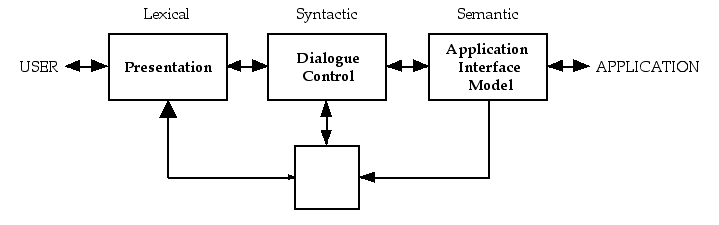
\includegraphics[width=125mm]{03/images/seeheim}
\end{figure}